\section{解析方法}
\subsection{波形の解析}
図\ref{fg:Lecroy_output} にオシロスコープの出力を示す。
オレンジ色の信号が赤外線パルスレーザー本体から取得したトリガー信号である。トリガーは1 MHzでthresholdは1.5 Vに設定した。
トリガー信号から出てから約55 ns後に見られる黄色の信号がLGADの信号である。
LGADの信号はアンプボードのノイズによって、0 mV付近でふらつく。
そのため、0 mVをベースラインとして、ベースラインと信号の最小値の差を波高とした。
信号サイズの違いによるタイムウォークの影響を小さくするために、波高の50%を閾値とした。
レーザーのトリガーと波高の50%を越えた時間差を信号の到達時間とした。

\begin{figure}[h]
    \centering
    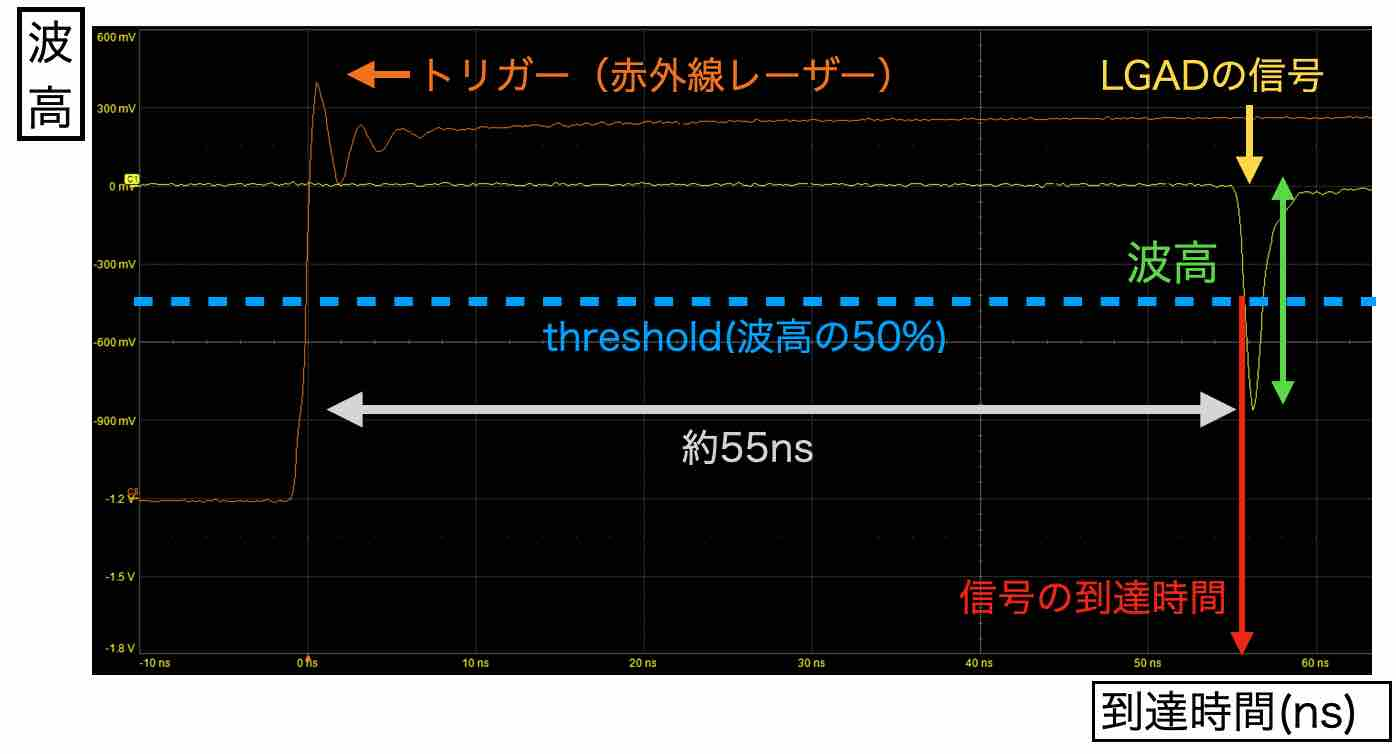
\includegraphics[width=15cm]{fig/ch4/Lecroy_output.jpg}
    \caption[オシロスコープの出力とデータの取得方法]{オシロスコープの出力とデータの取得方法\\横軸が時間、縦軸が波高である。トリガー(橙色)の55 ns後にLGADの信号(黄色)が来る。ベースラインとLGADの信号の最小値の差を波高、波高の50%の時の時間を到達時間とした。}
    \label{fg:Lecroy_output}
\end{figure}

\subsection{信号の大きさと時間分解能}
信号の大きさと時間分解能を測定するために、波形から取得した波高と到達時間のデータを用いて、
%図\ref{fg:phvstime} のようにx軸が到達時間、y軸が波高の2次元ヒストグラムを作成した。
図\ref{fg:Treso_hist} の到達時間のヒストグラムと
図\ref{fg:Ph_hist} の波高のヒストグラムを作成した。
時間分解能は到達時間のヒストグラムの標準偏差とした。標準偏差は到達時間のヒストグラムを、ガウス分布でフィッティングすることで求めた。
時間分解能には、レーザーのトリガーの10 ps未満のタイミングジッタの影響も含まれている。
信号の大きさは波高のヒストグラムの最頻値とした。最頻値は波高のヒストグラムを、非対称ガウス分布をフィットすることで求めた。
この解析を各電圧で行い、信号の大きさ、時間分解能、増幅率の電圧依存性を求めた。

LGADに関しては、逆電圧を印加し初めてから増幅層が空乏化するまで、信号は見えない。したがって、バルク部の空乏化が始まる70 V程度から、信号は見え始める。
そのため、LGADは70 Vから200 Vの範囲を測定した。PINに関しては、0 Vから200 Vの範囲を測定した。
また、時間分解能が良いと予想される180Vから200Vの範囲については、細かい電圧ステップで測定を行った。

LGADの信号の大きさを$S_{\rm{LGAD}}$とし、PINの信号の大きさを$S_{\rm{PIN}}$とすると、
増幅率は 式\ref{eq_Gain} のように、LGADの信号の大きさとPINの信号の大きさの比を取ることで、増幅層で電荷が何倍に増幅されるかを求めることができる。

\begin{equation}
    {Gain}(V) = \frac{S_{\rm{LGAD}}}{S_{\rm{PIN}}}
    \label{eq_Gain}
\end{equation}

%\begin{figure}[h]
%    \centering
%    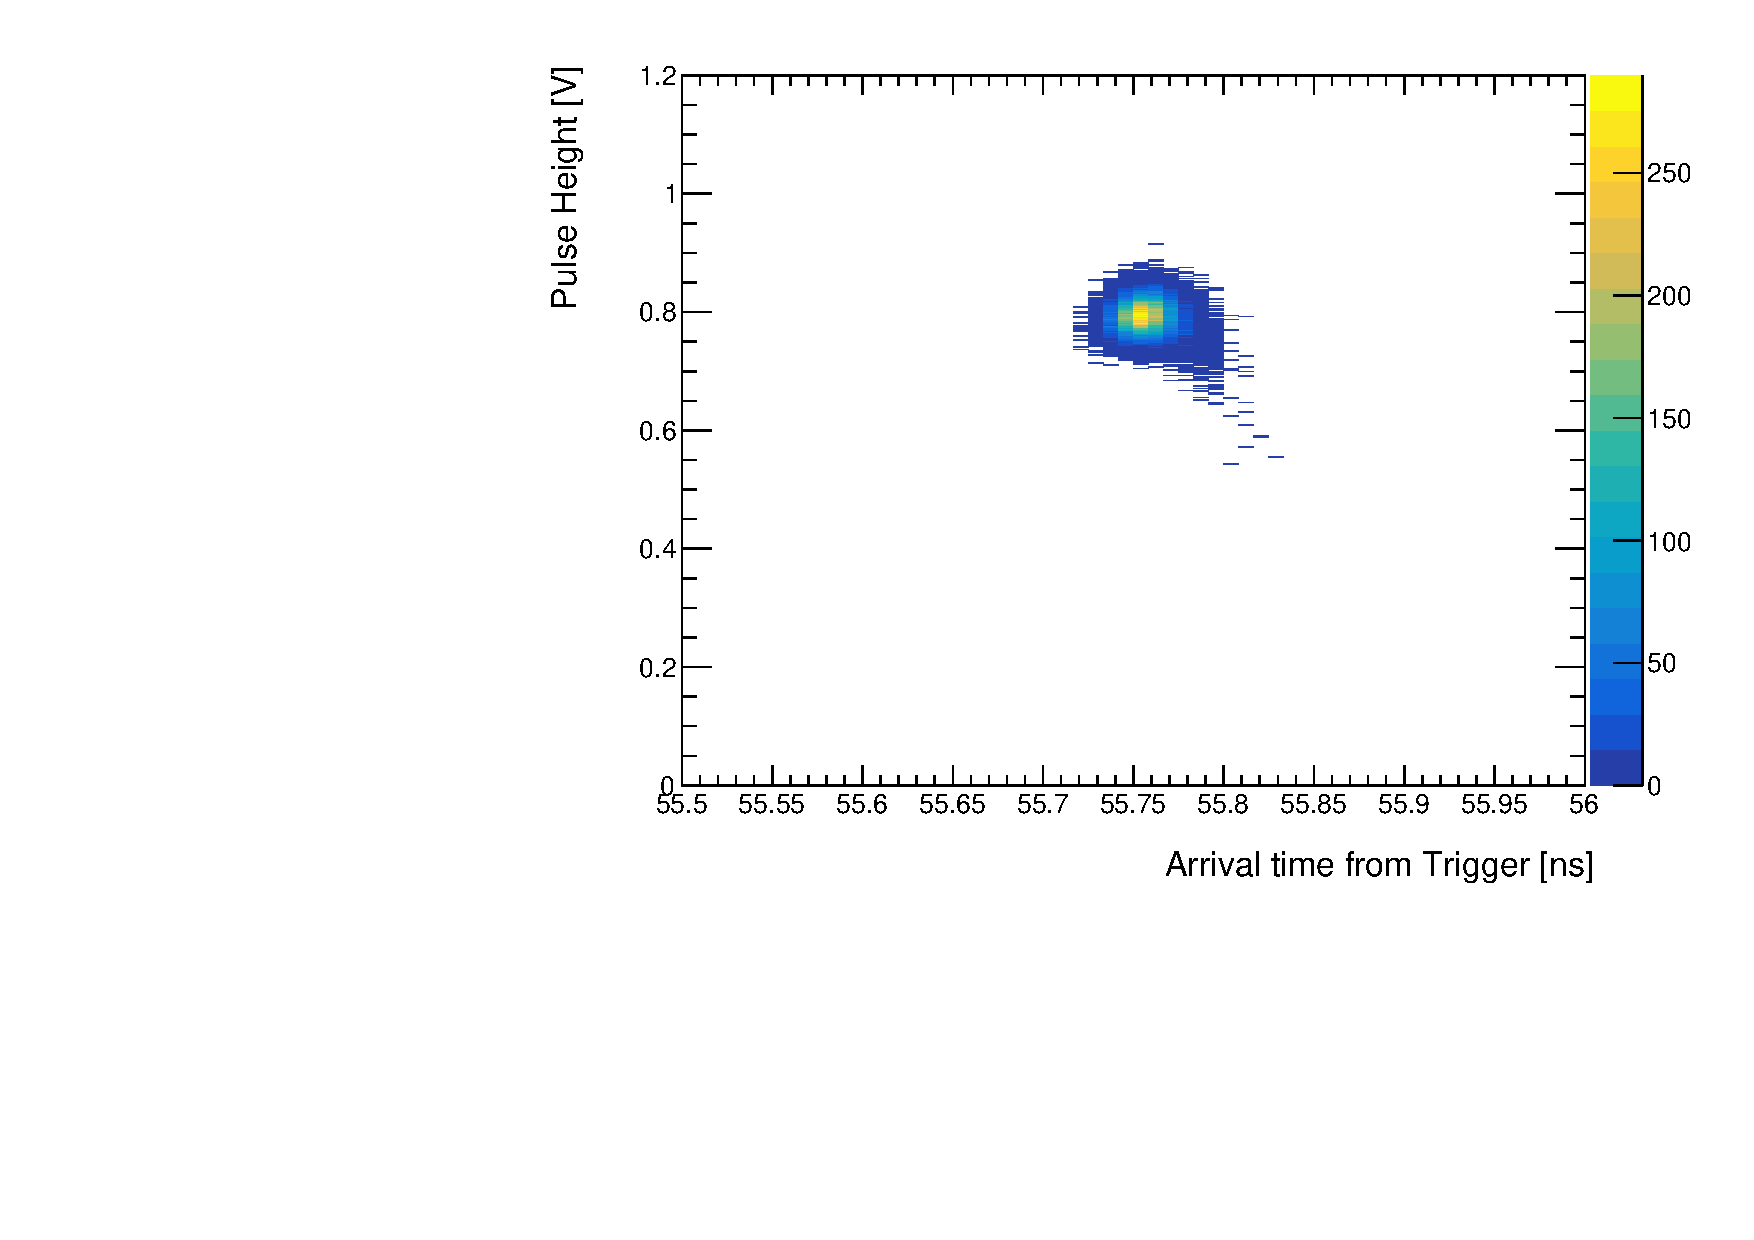
\includegraphics[width=10cm]{fig/graph/PhvsTime.pdf}
%    \caption[波高と到達時間の2次元ヒストグラム]{波高と到達時間の2次元ヒストグラム\\x軸が到達時間でy軸が波高}
%    \label{fg:phvstime}
%\end{figure}

\begin{figure}[h]
    \begin{minipage}[b]{0.5\linewidth}
        \centering
        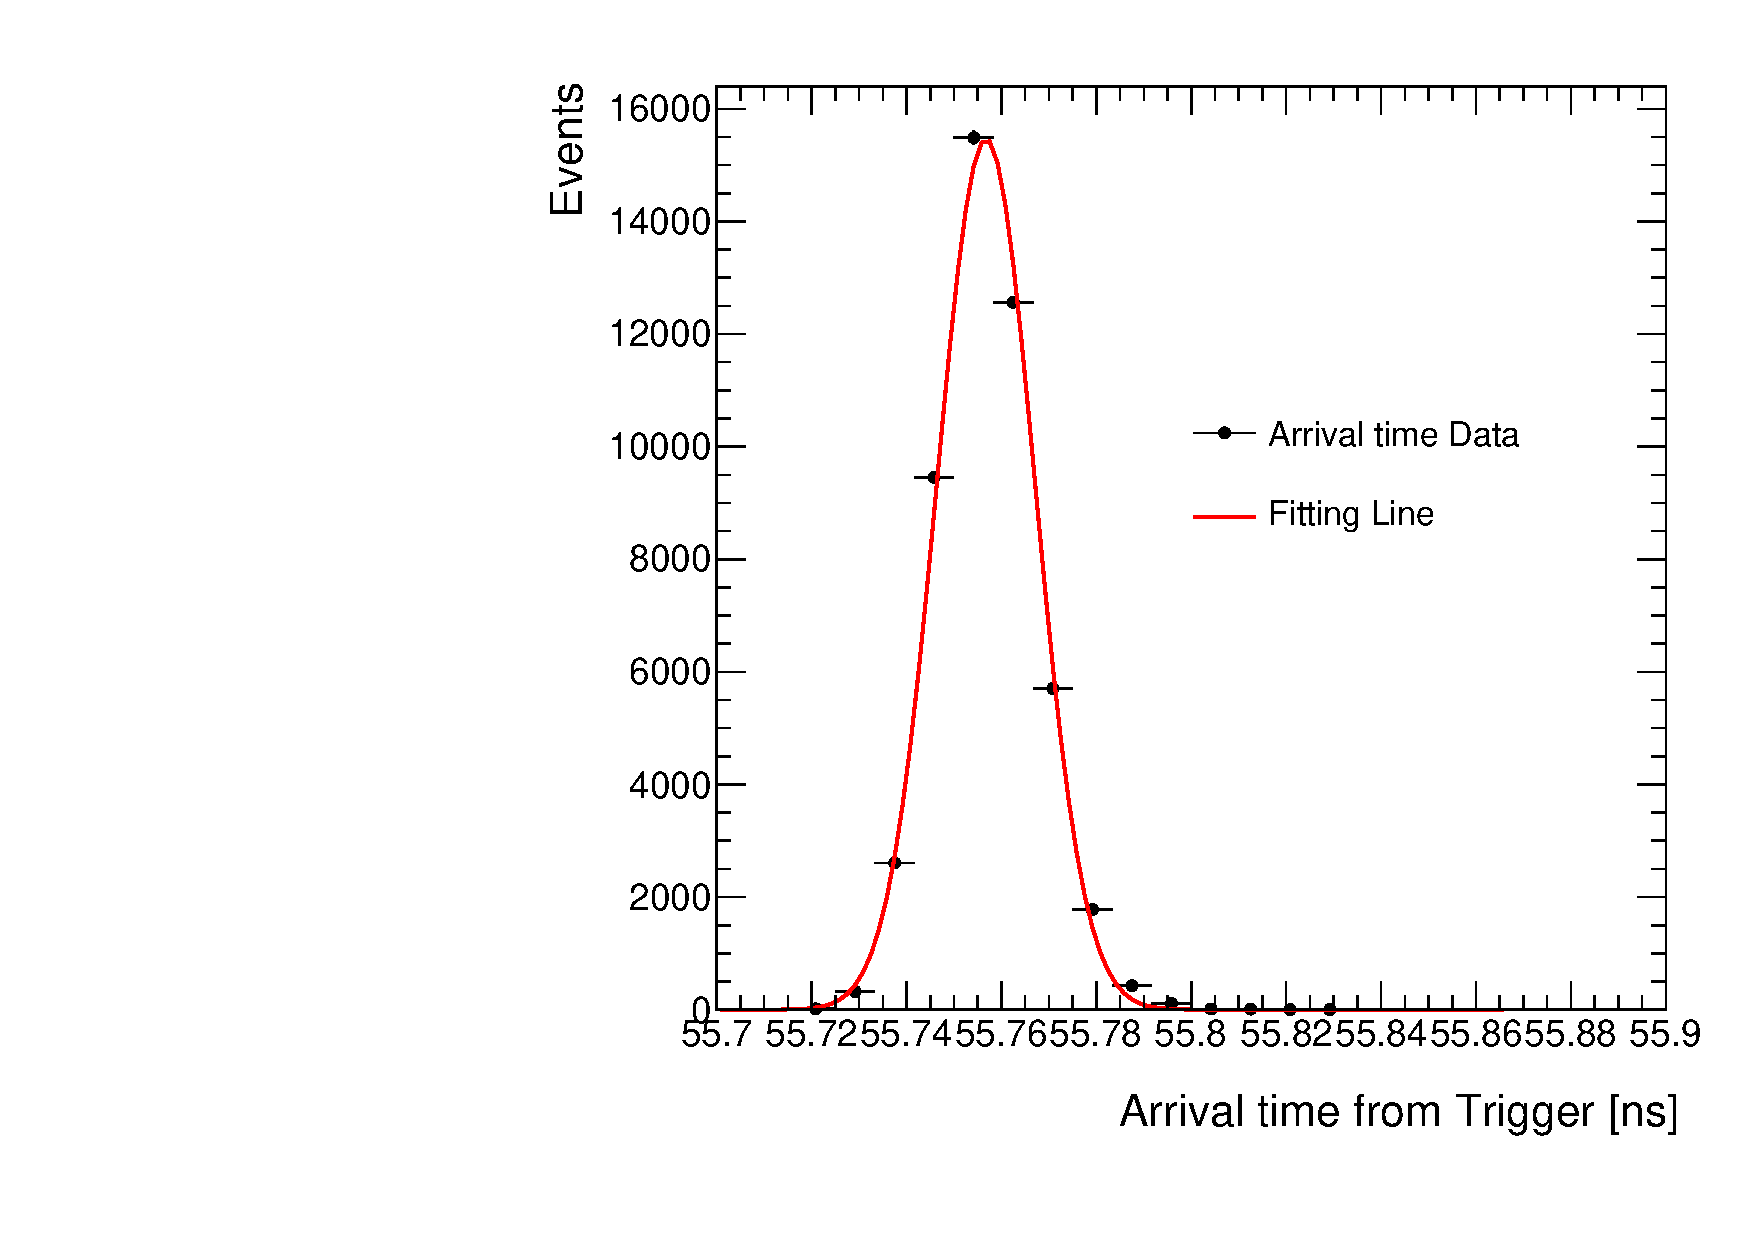
\includegraphics[width=8cm]{fig/graph/Treso_hist.pdf}
        \subcaption{到達時間}
        \label{fg:Treso_hist}
    \end{minipage}
    \begin{minipage}[b]{0.5\linewidth}
        \centering
        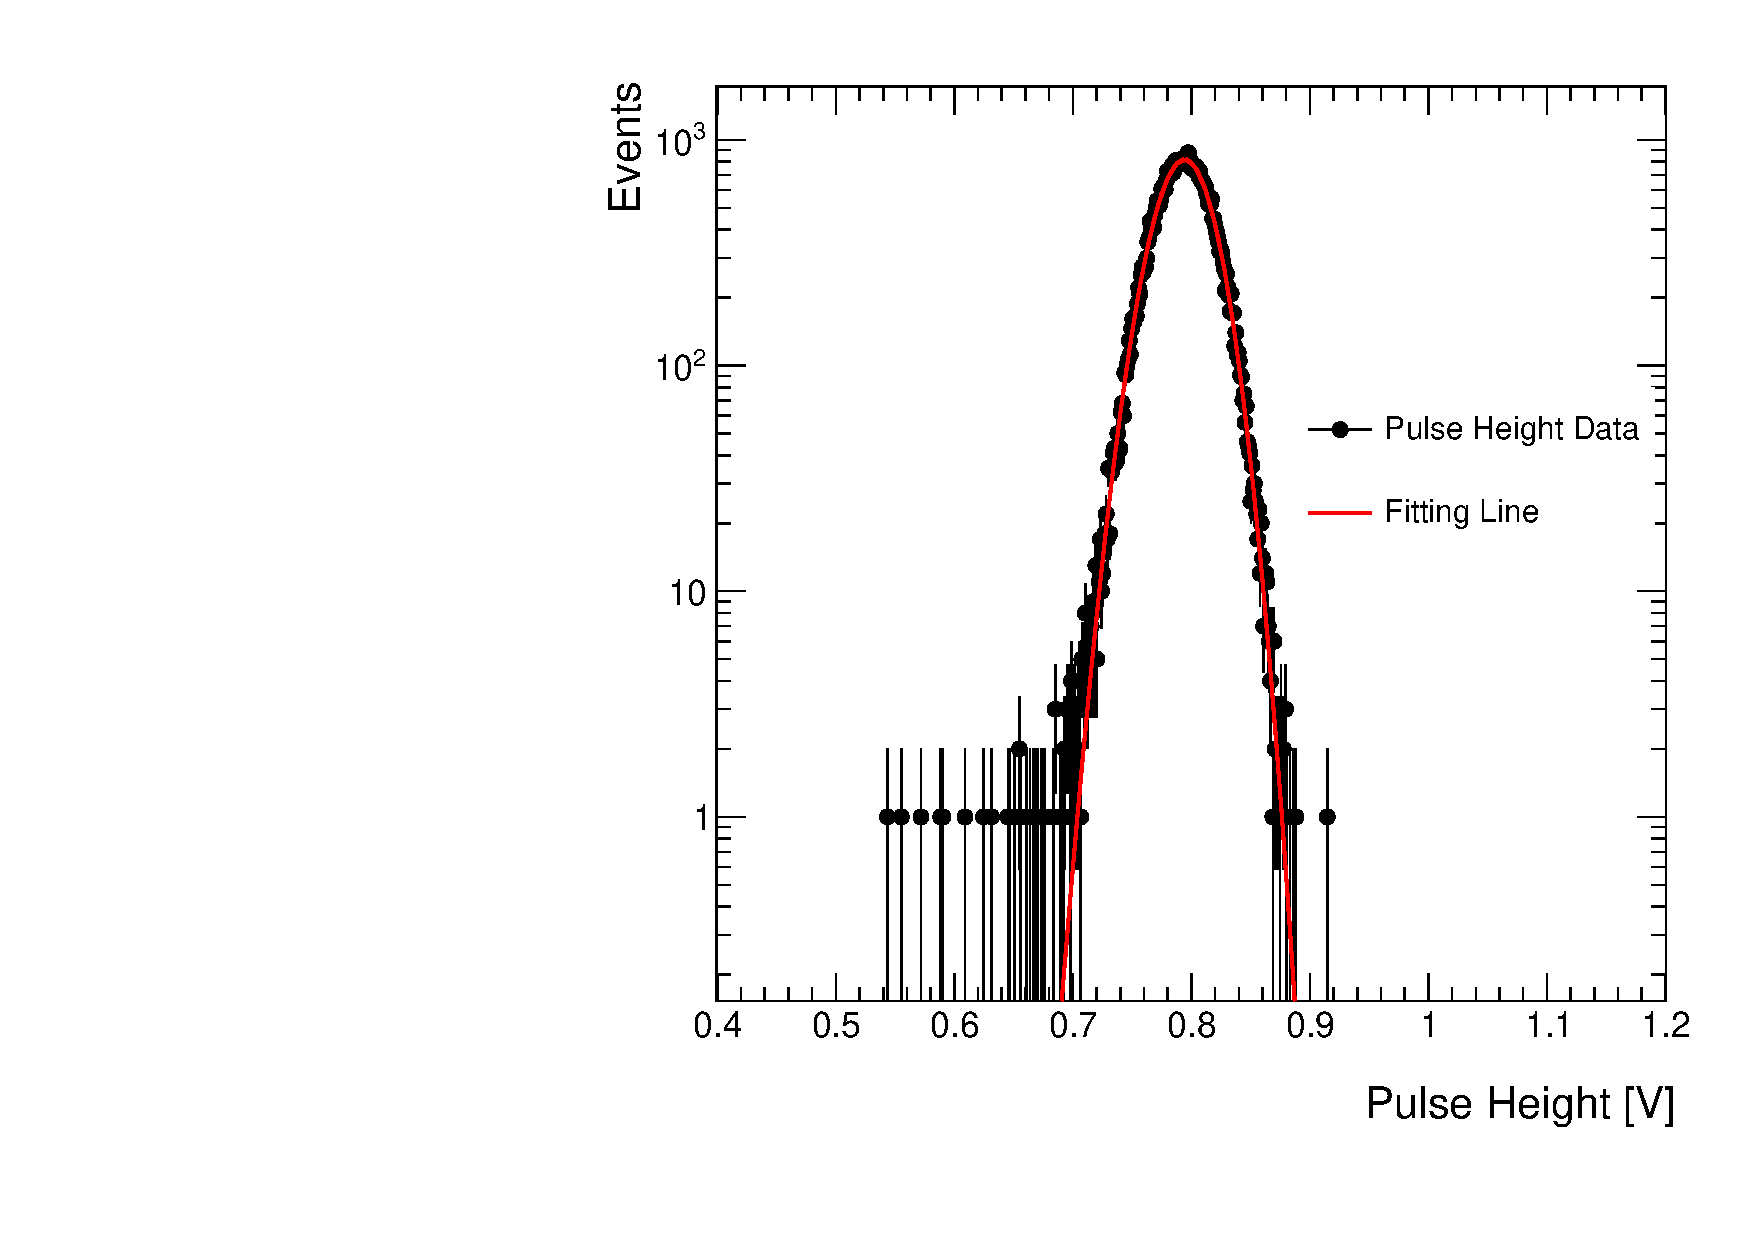
\includegraphics[width=8cm]{fig/graph/Ph_hist.pdf}
        \subcaption{波高}
        \label{fg:Ph_hist}
    \end{minipage}
    \caption[波高と到達時間のヒストグラム]{(a)が到達時間のヒストグラムで標準偏差を時間分解能とした。\\(b)が波高のヒストグラムで最頻値を信号の大きさとした。\\黒点が各データ点で赤線がフィッティングした結果}
\end{figure}


